\documentclass[a4paper]{article}
\usepackage[spanish]{babel}
\usepackage[utf8]{inputenc}
\usepackage{fancyhdr}
\usepackage{charter} % tipografia
%\usepackage{graphicx}
\usepackage[pdftex]{graphicx}
\usepackage{bm} % bold font in math mode
\usepackage{sidecap}
\usepackage{caption}
\usepackage{subcaption}
\usepackage{booktabs}
\usepackage{makeidx}
\usepackage{float}
\usepackage{amsmath, amsthm, amssymb}
\newtheorem{theorem}{Teorema}
\newtheorem{customthm}{Teorema}
\newtheorem{corollary}{Corolario}[theorem]
\newtheorem{proposition}[theorem]{Proposición}
\newtheorem{innercustomlemma}{Lemma}
\newenvironment{customlemma}[1]
  {\renewcommand\theinnercustomlemma{#1}\innercustomlemma}
  {\endinnercustomlemma}
\usepackage{amsfonts}
\usepackage{sectsty}
\usepackage{charter}
\usepackage{wrapfig}
\usepackage{listings}
\usepackage{hyperref} % links
\usepackage{algorithm} %http://www.ctan.org/pkg/algorithms
\usepackage{algorithmic}
\usepackage[usenames,dvipsnames]{xcolor}
\usepackage{pgfplots}
% \usepackage{pgfplotstable}
% custom
\usepackage{color} % para snipets de codigo coloreados
\usepackage{fancybox} % para el sbox de los snipets de codigo
\definecolor{litegrey}{gray}{0.94}
% \newenvironment{sidebar}{%
% \begin{Sbox}\begin{minipage}{.85\textwidth}}%
% {\end{minipage}\end{Sbox}%
% \begin{center}\setlength{\fboxsep}{6pt}%
% \shadowbox{\TheSbox}\end{center}}
% \newenvironment{warning}{%
% \begin{Sbox}\begin{minipage}{.85\textwidth}\sffamily\lite\small\RaggedRight}%
% {\end{minipage}\end{Sbox}%
% \begin{center}\setlength{\fboxsep}{6pt}%
% \colorbox{litegrey}{\TheSbox}\end{center}}

%\newenvironment{codesnippet}{%
%\begin{Sbox}\begin{minipage}{\linewidth-2\fboxsep-2\fboxrule-4pt}\sffamily\small}%
%{\end{minipage}\end{Sbox}%
%\begin{center}%
%\colorbox{litegrey}{\TheSbox}\end{center}}

% \newenvironment{codesnippet}{\VerbatimEnvironment%
%   \noindent
%   %{\columnwidth-\leftmargin-\rightmargin-2\fboxsep-2\fboxrule-4pt}
%   \begin{Sbox}
%   \begin{minipage}{\linewidth-2\fboxsep-2\fboxrule-4pt}
%   \begin{Verbatim}
% }{%
%   \end{Verbatim}
%   \end{minipage}
%   \end{Sbox}%
%   \colorbox{litegrey}{\TheSbox}
% }

\newenvironment{codesnippet}{\VerbatimEnvironment%
  \noindent
  %      {\columnwidth-\leftmargin-\rightmargin-2\fboxsep-2\fboxrule-4pt}
  \begin{Sbox}
  \begin{minipage}{\linewidth}
  \begin{Verbatim}
}{%
  \end{Verbatim}
  \end{minipage}
  \end{Sbox}%
  \colorbox{litegrey}{\TheSbox}
}

\usepackage{fancyhdr}
\pagestyle{fancy}
%\renewcommand{\chaptermark}[1]{\markboth{#1}{}}
\renewcommand{\sectionmark}[1]{\markright{\thesection\ - #1}}
\fancyhf{}
\fancyhead[LO]{Sección \rightmark} % \thesection\
\fancyfoot[LO]{\small{Iv\'an Arcuschin, Mart\'in Jedwabny, Jos\'e Massigoge, Iv\'an Pondal}}
\fancyfoot[RO]{\thepage}
\renewcommand{\headrulewidth}{0.5pt}
\renewcommand{\footrulewidth}{0.5pt}
\setlength{\hoffset}{-0.8in}
\setlength{\textwidth}{16cm}
%\setlength{\hoffset}{-1.1cm}
%\setlength{\textwidth}{16cm}
\setlength{\headsep}{0.5cm}
\setlength{\textheight}{25cm}
\setlength{\voffset}{-0.7in}
\setlength{\headwidth}{\textwidth}
\setlength{\headheight}{13.1pt}
\renewcommand{\baselinestretch}{1.1} % line spacing

% -------------------- COMANDOS ESPECIALES ------------------------------

\newcommand{\calcular}[2]{\pgfmathtruncatemacro{#1}{#2}}

\pgfplotsset{
  filter params/.style n args={4}{
      x filter/.code={
          \edef\tempa{\thisrow{#1}}
          \edef\tempb{#2}
          \edef\tempc{\thisrow{#3}}
          \edef\tempd{#4}
          \ifx\tempa\tempb
            \ifx\tempc\tempd
            \else
              \def\pgfmathresult{inf}
            \fi
          \else
            \def\pgfmathresult{inf}
          \fi
      }
  }
}

\newcommand{\graficarDatos}[6]{
  \begin{tikzpicture}
  \begin{axis}[
      title={#1},
      xlabel={#2},
      ylabel={#3},
      scaled x ticks=false,
      scaled y ticks=false,
      scale=0.5
  ]
  \addplot[only marks, color=black] table[x=#4,y=#5]{#6};
  \end{axis}
  \end{tikzpicture}
}

\newcommand{\graficarDatosPlus}[7]{
  \begin{tikzpicture}
  \begin{axis}[
      title={#1},
      xlabel={#2},
      ylabel={#3},
      scaled x ticks=false,
      scaled y ticks=false,
      width=0.6\textwidth,
      #7
  ]
  \addplot[only marks, color=black] table[x=#4,y=#5]{#6};
  \end{axis}
  \end{tikzpicture}
}

\makeatletter
\pgfplotsset{
    groupplot xlabel/.initial={},
    every groupplot x label/.style={
        at={($({group c1r\pgfplots@group@rows.west}|-{group c1r\pgfplots@group@rows.outer south})!0.5!({group c\pgfplots@group@columns r\pgfplots@group@rows.east}|-{group c\pgfplots@group@columns r\pgfplots@group@rows.outer south})$)},
        anchor=north,
    },
    groupplot ylabel/.initial={},
    every groupplot y label/.style={
            rotate=90,
        at={($({group c1r1.north}-|{group c1r1.outer
west})!0.5!({group c1r\pgfplots@group@rows.south}-|{group c1r\pgfplots@group@rows.outer west})$)},
        anchor=south
    },
    execute at end groupplot/.code={%
      \node [/pgfplots/every groupplot x label]
{\pgfkeysvalueof{/pgfplots/groupplot xlabel}};
      \node [/pgfplots/every groupplot y label]
{\pgfkeysvalueof{/pgfplots/groupplot ylabel}};
    },
    group/only outer labels/.style =
{
group/every plot/.code = {%
    \ifnum\pgfplots@group@current@row=\pgfplots@group@rows\else%
        \pgfkeys{xticklabels = {}, xlabel = {}}\fi%
    \ifnum\pgfplots@group@current@column=1\else%
        \pgfkeys{yticklabels = {}, ylabel = {}}\fi%
}
}
}

\def\endpgfplots@environment@groupplot{%
    \endpgfplots@environment@opt%
    \pgfkeys{/pgfplots/execute at end groupplot}%
    \endgroup%
}
\makeatother

\newcommand{\barGraphExp}[2]{
    \begin{tikzpicture}
    \begin{axis}[
        xlabel={Implementación},
    	ylabel={Tiempo de ejecución (clocks)},
        legend style={at={(1.4,1.0)}},
        ybar,
        scaled ticks=false,
        width=0.5\textwidth,
        height=0.5\textwidth,
        tickpos=left,
        xtick=\empty,
        ytick align=inside,
        xtick align=inside,
    	enlargelimits=0.05,
        bar width=16,
    ]
    % How to process each item:
    \renewcommand*{\do}[1]{\addplot+[color=black] table[x=n, y=##1]{datos/datos_blur.dat};}
    % Process list:
    \docsvlist{#2}
    \legend{#2}
    \end{axis}
    \end{tikzpicture}
}

\newcommand{\graficarDatosExp}[6]{
  \begin{tikzpicture}
  \begin{axis}[
      title={#1},
      xlabel={#2},
      ylabel={#3},
      scaled x ticks=false,
      scaled y ticks=false,
      enlargelimits=0.05,
      width=0.5\textwidth,
      height=0.5\textwidth
  ]
  \addplot[color=black] table[x=#5,y=#6]{#4};
  % \renewcommand*{\do}[1]{\addplot table[x=#5,y=##1]{#4};}
  % %     % Process list:
  % \docsvlist{#6}
  % \legend{#6}
  \end{axis}
  \end{tikzpicture}
}

% ------------------------------------------------------------------------

% \setcounter{secnumdepth}{2}
\usepackage{underscore}
\usepackage{kbordermatrix}% Matrix column labels
\usepackage{caratula}
\usepackage{url}
\lstset{
    language=C++,
    basicstyle=\ttfamily,
    keywordstyle=\color{blue}\ttfamily,
    stringstyle=\color{red}\ttfamily,
    commentstyle=\color{ForestGreen}\ttfamily,
    morecomment=[l][\color{magenta}]{\#}
}

% *********************** %
\usepackage{tikz}
\usetikzlibrary{graphs}
\usetikzlibrary{calc}
\usetikzlibrary{arrows}
% Otros
\usepackage{arrayjobx}
\usepackage{enumitem}
\usepackage{multicol}
\usepackage{etoolbox}
%\newcommand{\noindex}{\hspace*{-0.8em}}%
\lstset{breaklines=true}
\newcommand{\subscript}[2]{$#1 _ #2$}
% *********************** %

% ******************************************************** %
% TEMPLATE DE INFORME ORGA2 v0.1 %
% ******************************************************** %
% ******************************************************** %
% %
% ALGUNOS PAQUETES REQUERIDOS (EN UBUNTU): %
% ========================================
% %
% texlive-latex-base %
% texlive-latex-recommended %
% texlive-fonts-recommended %
% texlive-latex-extra %
% texlive-lang-spanish (en ubuntu 13.10) %
% ******************************************************** %
\begin{document}
\thispagestyle{empty}
\materia{Métodos Numéricos}
\submateria{Segundo Cuatrimestre de 2015}
\titulo{Trabajo Práctico I}
%\subtitulo{Grupo: }
\integrante{Iv\'an Arcuschin}{678/13}{iarcuschin@gmail.com}
\integrante{Mart\'in Jedwabny}{885/13}{martiniedva@gmail.com}
\integrante{Jos\'e Massigoge}{954/12}{jmmassigoge@gmail.com}
\integrante{Iv\'an Pondal}{???/??}{ivan.pondal@gmail.com}
\maketitle
% no footer on the first page
\thispagestyle{empty}
\newpage

\tableofcontents

\newpage
\section{Introducción}
El objetivo de este Trabajo Práctico es implmentar diferentes algoritmos de resolución de sistemas de ecuaciones lineales y experimentar con dichas implementaciones en el contexto de un problema de la vida real.

El problema a resolver es hallar la isoterma 500C en la pared de un Alto Horno. Para tal fin, deberemos particionar la pared del horno en puntos finitos, y luego resolver un sistema de ecuaciones lineales, en el cual cada punto de la pared interior y exterior del Horno es un dato, y las ecuaciones para los puntos internos satisfacen la ecuación del calor.

Los experimentos realizados se dividen en dos partes: Comportamiento del sistema y Evaluación de los métodos. En la primera parte, analizaremos con los  distintas instancias de prueba y se estudiará la proximidad de la isoterma buscada respecto de la pared exterior del horno. En la segunda parte, analizaremos el tiempo de computo requerido para la resolución del sistema en función de la granularidad de la discretización y analizaremos el escenario en el cual las temperaturas de los bordes varian a lo largo del tiempo.


\newpage
\section{Modelo}
\subsection{Descripción}

El Alto Horno está definido por las siguientes variables:
\begin{itemize}
    \item El radio de la pared exterior: $r_e \in \mathbb{R}$
    \item El radio de la pared interior: $r_i \in \mathbb{R}$
    \item La temperatura en cada punto de la pared:  $T(r,\theta)$, donde $(r,\theta)$ se encuentra expresado en coordenadas polares, siendo $r$ el radio y $\theta$ el \'angulo polar de dicho punto.

    Son datos del problema, las temperaturas de la pared interior y exterior:
    \begin{itemize}
        \item $T(r_i,\theta) = T_i \;\;\;\;\;para\;todo\;punto\;(r,\theta)\;con\;r\leq r_i$
        \item $T(r_e,\theta) = T_e(\theta) \;\;\;\;\;\;para\;todo\;punto\;(r_e,\theta)$
    \end{itemize}
\end{itemize}

La Figura 1 muestra las variables al tomar una sección circular del horno.

\begin{figure}[ht]
\begin{center}
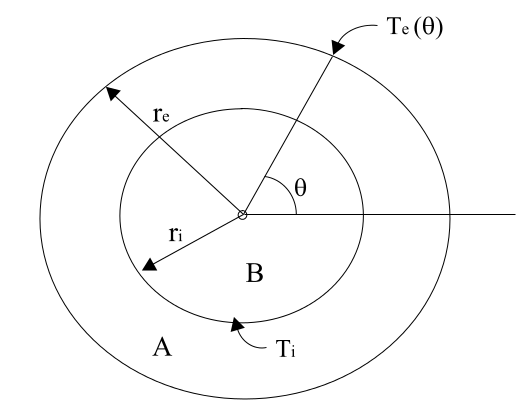
\includegraphics[width=0.6\columnwidth]{imagenes/horno.png}
\caption{Secci\'on circular del horno}
\end{center}
\end{figure}

En el estado estacionario, cada punto de la pared satisface la ecuación del calor:

\begin{equation}\label{calor}
\frac{\partial^2T(r,\theta)}{\partial r^2}+\frac{1}{r}\frac{\partial T(r,\theta)}{\partial r}+\frac{1}{r^2}\frac{\partial^2T(r,\theta)}{\partial \theta^2} = 0
\end{equation}

\medskip

Para resolver este problema computacionalmente, discretizamos el dominio del problema (el sector A) en coordenadas polares. Consideramos una partici\'on $0 = \theta_0 < \theta_1 < ... < \theta_n = 2\pi$ en $n$ \'angulos discretos con $\theta_k-\theta_{k-1} = \Delta\theta$ para $k = 1,...,n$, y una partici\'on $r_i = r_0 < r_1 < ... < r_m = r_e$ en $m+1$ radios discretos con $r_j - r_{j-1} = \Delta r$ para $j = 1,...,m$.

\medskip

El problema ahora consiste en determinar el valor de la funci\'on $T$ en los puntos de la discretizaci\'on $(r_j,\theta_k)$ que se encuentren dentro del sector A. Llamemos $t_{jk} = T(r_j,\theta_k)$ al valor (desconocido) de la funci\'on $T$ en el punto $(r_j,\theta_k)$.

\medskip

Para encontrar estos valores, transformamos la ecuaci\'on (\ref{calor}) en un conjunto de ecuaciones lineales sobre las inc\'ognitas $t_{jk}$, evaluando (\ref{calor}) en todos los puntos de la discretizaci\'on que se encuentren dentro del sector A. Al hacer esta evaluaci\'on, aproximamos las derivadas parciales de $T$ en (\ref{calor}) por medio de las siguientes f\'ormulas de diferencias finitas:


\begin{equation}
\frac{\partial^2T(r,\theta)}{\partial r^2}(r_j,\theta_k) \cong \frac{t_{j-1,k}-2t_{jk}+t_{j+1,k}}{(\Delta r)^2}
\end{equation}

\begin{equation}
\frac{\partial T(r,\theta)}{\partial r}(r_j,\theta_k) \cong \frac{t_{j,k}-t_{j-1,k}}{\Delta r}
\end{equation}

\begin{equation}
\frac{\partial^2T(r,\theta)}{\partial \theta^2}(r_j,\theta_k) \cong \frac{t_{j,k-1}-2t_{jk}+t_{j,k+1}}{(\Delta \theta)^2}
\end{equation}


\subsection{Representación del sistema}

Para representar el sistema de ecuaciones presentado, se utilizará una matriz simple, implementada como un vector de vectores. A continuación, se muestra como quedaría la matriz para las ecuaciones de los puntos $t_{0,0}, t_{0,n-1}, t_{i,j}, t_{m,0}$ y $t_{m,n-1}$.

\[
    % reduce columns padding:
    \setlength{\arraycolsep}{1pt}
    % fila vertical alternativa:
    % \vdots   &  \multicolumn{6}{c}{\strut}      &\vdots&         \multicolumn{6}{c}{}               & \vrule & {} \\
    \kbordermatrix{%
                       & \bm{t_{0,0}} & \ldots & \bm{t_{0,n-1}} & \ldots & t_{i-1,j}           & \ldots & t_{i,j-1}   & \bm{t_{i,j}}                & t_{i,j+1}   & \ldots & t_{i+1,j}   & \ldots & \bm{t_{m,0}} & \ldots & \bm{t_{m,n-1}} &        & b        \\
        \bm{t_{0,0}}   & 1            & \ldots & 0              & \ldots & 0                   & \ldots & 0           & 0                           & 0           & \ldots & 0           & \ldots & 0            & \ldots & 0              & \vrule & t_{0,0}   \\
        \vdots         & \vdots       & {}     & \vdots         & {}     & \vdots              & {}     & \vdots      & \vdots                      & \vdots      & {}     & \vdots      & {}     & \vdots       & {}     & \vdots         & \vrule & {}       \\
        \bm{t_{0,n-1}} & 0            & \ldots & 1              & \ldots & 0                   & \ldots & 0           & 0                           & 0           & \ldots & 0           & \ldots & 0            & \ldots & 0              & \vrule & t_{0,n-1} \\
        \vdots         & \vdots       & {}     & \vdots         & {}     & \vdots              & {}     & \vdots      & \vdots                      & \vdots      & {}     & \vdots      & {}     & \vdots       & {}     & \vdots         & \vrule & {}       \\
        \bm{t_{i,j}}   & 0            & \ldots & 0              & \ldots & \bm{\beta - \gamma} & \ldots & \bm{\alpha} & \bm{-2\alpha-2\beta+\gamma} & \bm{\alpha} & \ldots & \bm{\beta}  & \ldots & 0            & \ldots & 0              & \vrule & 0        \\
        \vdots         & \vdots       & {}     & \vdots         & {}     & \vdots              & {}     & \vdots      & \vdots                      & \vdots      & {}     & \vdots      & {}     & \vdots       & {}     & \vdots         & \vrule & {}       \\
        \bm{t_{m,0}}   & 0            & \ldots & 0              & \ldots & 0                   & \ldots & 0           & 0                           & 0           & \ldots & 0           & \ldots & 1            & \ldots & 0              & \vrule & t_{m,0}   \\
        \vdots         & \vdots       & {}     & \vdots         & {}     & \vdots              & {}     & \vdots      & \vdots                      & \vdots      & {}     & \vdots      & {}     & \vdots       & {}     & \vdots         & \vrule & {}       \\
        \bm{t_{m,n-1}} & 0            & \ldots & 0              & \ldots & 0                   & \ldots & 0           & 0                           & 0           & \ldots & 0           & \ldots & 0            & \ldots & 1              & \vrule & t_{m,n-1}
    }
\]

Donde,
\begin{itemize}
    \item $\alpha = \frac{1}{(\Delta\theta)^2 * r^2}$
    \item $\beta = \frac{1}{(\Delta\ r)^2}$
    \item $\gamma = \frac{1}{(\Delta\ r) * r}$
    \item $0 < i < n$
    \item $0 < j < m+1$
\end{itemize}

\medskip

Notese que la ecuación del punto $t_{i,j}$ tiene ceros en todas sus celdas, excepto en las corresponiendentes a $t_{i-1,j}$, $t_{i,j}$, $t_{i+1j0}$, $t_{i,j-1}$ y $t_{i,j+1}$.
Se puede ver que para cada fila de la matriz, hay una ``banda'' de tamaño $2n$ alrededor de la diagonal donde hay 5 elementos que no son cero.


\newpage
\section{Demostración: Eliminación Gaussiana sin pivoteo}
\begin{proposition}
    Sea $A \in \mathbb{R}^{n(m+1) \times n(m+1)}$ la matriz obtenida para el sistema definido por las ecuaciones del Modelo, en donde $m+1$ y $n$ corresponden a la cantidad de radios y angulos respectivamente de la discretizacion. Demostrar que es posible aplicar Eliminación Gaussiana sin pivoteo.
\end{proposition}

Para poder demostrar la proposición, utilizamos los siguientes lemas, que demostramos a continuacion:

  \begin{enumerate}[label=(\subscript{L}{\arabic*})]
    \item $A$ es una matriz banda.
    \item $A$ es diagonal dominante (no estricta).

  \end{enumerate}

  \begin{customlemma}{$L_{1}$}
    $A$ es una matriz banda
  \end{customlemma}

  \begin{proof}
    A partir del Modelo descripto en el punto anterior, vease figura \ref{fig:matriz}, podemos concluir que $A$ es una matriz banda.
  \end{proof}

  \begin{customlemma}{$L_{2}$}
    $A$ es diagonal dominante (no estricta).
  \end{customlemma}

  \begin{proof}
    Por definición, una matriz es diagonal dominante (no estrictamente) cuando se cumple que, $\forall i = 0,1,...,n-1$:
    \begin{equation*}
        \begin{aligned}
          |a_{i,i}| &\geq \sum\limits_{\substack{j=0  \\ j \neq i}}^{n-1} |a_{i,j}| \\
        \end{aligned}
    \end{equation*}
    Esta desigualdad es evidente para las primeras  y ultimas $n$ filas, ya que el unico valor distinto de 0 se encuentra en la diagonal.
    Falta ver el caso para el resto de $A$. Tenemos que probar que para fila, $i$, se cumple:
    \begin{equation*}
        \begin{aligned}
          |-2\alpha-2\beta+\gamma| \geq |\beta - \gamma| + |\alpha| + |\alpha| + |\beta|
        \end{aligned}
    \end{equation*}
    \newline
    Recordando que: $\alpha = \frac{1}{(\Delta\theta)^2 * r^2}$, $\beta = \frac{1}{(\Delta\ r)^2}$ y $\gamma = \frac{1}{(\Delta\ r) * r}$.
    \newline
    \newline
    Entonces, por definicion sabemos que $|\alpha| = \alpha$ y $|\beta| = \beta$.
    \newline
    \newline
    Veamos que $|\beta - \gamma| = \beta - \gamma$. Supongamos que $\beta - \gamma < 0$:

    \begin{equation*}
        \begin{aligned}
          \beta &< \gamma \\
          %\text{Por definicion de  $\beta$ y $\gamma$:} \\
          \frac{1}{(\Delta\ r)^2}  &< \frac{1}{(\Delta\ r) * r_{j}} \\
          1 &< \frac{\Delta\ r}{r_{j}} \\
          %\text{Sabemos que } \Delta\ r = r_{j} - r_{j-1} \text{ para $j=1,...,m$. Reemplazando:} \\
          1 &< \frac{r_{j} - r_{j-1}}{r_{j}} \\
          1 &< 1 - \frac{r_{j-1}}{r_{j}} \\
          %\text{ Como los radios son todos mayores a 0, llegamos a un absurdo, que vino de suponer }\beta - \gamma &< 0, \text{por lo tanto }\beta - \gamma \geq 0.
        \end{aligned}
    \end{equation*}
    Como los radios son todos mayores a 0, llegamos a un absurdo, que vino de suponer $\beta - \gamma < 0$, por lo tanto $\beta - \gamma \geq 0$.
    \newline
    \newline
    Deberiamos probar que la desigualdad se cumple para los siguientes casos:

    \begin{enumerate}
      \item $-2\alpha-2\beta+\gamma \geq 0$
      \item $-2\alpha-2\beta+\gamma < 0$
    \end{enumerate}
    Veamos caso por caso:
    \begin{enumerate}
      \item \bm{$-2\alpha-2\beta+\gamma \geq 0$}:

        \begin{equation*}
          \begin{aligned}
          -2\alpha-2\beta+\gamma &\geq \beta - \gamma + \alpha + \alpha + \beta \\
           2\gamma &\geq 4\beta + 4\alpha \\
           \gamma &\geq 2\beta + 2\alpha \\
           \gamma - 2\beta - 2\alpha& \geq 0
          \end{aligned}
        \end{equation*}
        Que vale por ser exactamente la hipótesis del caso 1.

      \item \bm{$-2\alpha-2\beta+\gamma < 0$}:

        \begin{equation*}
          \begin{aligned}
           -2\alpha-2\beta+\gamma &\leq -\beta+\gamma-\alpha-\alpha-\beta \\
           \gamma - \gamma &\leq 2\beta - 2\beta + 2\alpha - 2\alpha \\
           0 &\leq 0
          \end{aligned}
        \end{equation*}

        Que vale siempre.

    \end{enumerate}


  \end{proof}

\begin{proof}[Demostración Proposición 1.]

Por $L_{2}$ sabemos que $A$ es diagonal dominante (no estricta) y por definicion del Modelo sabemos que $a_{0,0} = 1$.

Sea $A^{(1)}$ la matriz resultante luego de aplicar un paso de la Eliminación Gaussiana. Para toda fila $i = 1,...,n-1$ se cumple que:

\begin{equation*}
    \begin{aligned}
      a^{(1)}_{i,j} &= a^{(0)}_{i,j} - \frac{a^{(0)}_{0,j}a^{(0)}_{i,j}}{a^{(0)}_{0,0}}, \text{para } 1 \leq j \leq n(m+1)-1
    \end{aligned}
\end{equation*}

Sabemos que $a^{(1)}_{i,0} = 0$. Luego:

\begin{equation*}
    \begin{aligned}
      \sum\limits_{\substack{j=1  \\ j \neq i}}^{n(m+1)-1} |a^{1}_{i,j}| &= \sum\limits_{\substack{j=1  \\ j \neq i}}^{n(m+1)-1} |a^{(0)}_{i,j} - \frac{a^{(0)}_{0,j}a^{(0)}_{i,0}}{a^{(0)}_{0,0}}| \\
      &\leq \sum\limits_{\substack{j=1  \\ j \neq i}}^{n(m+1)-1} |a^{(0)}_{i,j}| + \sum\limits_{\substack{j=1  \\ j \neq i}}^{n(m+1)-1} |\frac{a^{(0)}_{0,j}a^{(0)}_{i,0}}{a^{(0)}_{0,0}}| \\
      &\leq |a^{(0)}_{i,i}| - |a^{(0)}_{i,0}| +  \frac{|a^{(0)}_{i,0}|}{|a^{(0)}_{0,0}|} \sum\limits_{\substack{j=1  \\ j \neq i}}^{n(m+1)-1} |a^{(0)}_{0,j}| \\
      &\leq |a^{(0)}_{i,i}| - |a^{(0)}_{i,0}| +  \frac{|a^{(0)}_{i,0}|}{|a^{(0)}_{0,0}|} (|a^{(0)}_{0,0}| - |a^{(0)}_{0,i}|) \\
      &= |a^{(0)}_{i,i}| - \frac{|a^{(0)}_{i,0}||a^{(0)}_{0,i}|}{|a^{(0)}_{0,0}|} \\
      &\leq |a^{(0)}_{i,i} - \frac{a^{(0)}_{i,0}a^{(0)}_{0,i}}{a^{(0)}_{0,0}}| = |a^{(1)}_{i,i}|
    \end{aligned}
\end{equation*}

\begin{itemize}
\item Por lo tanto, el dominio diagonal no estricto se establece en los renglones $1,..,n-1$, y como el primer renglon de $A^{(1)}$ y de $A$ son iguales,
$A^{(1)}$ sera diagonal dominante no estricto.

\item Para poder aplicar un paso más de la Eliminación Gaussiana, es necesario que $a^{(1)}_{1,1} \neq 0$. Sabemos por definición del Modelo que $a^{(0)}_{1,1} = 1$, y como $a^{(0)}_{1,0} = 0$, por definición de la Eliminación Gaussiana $a^{(1)}_{1,1} = 1$. Esta situación se repite para las $n$ primeras flas de $A$, ya que para $\forall i=0,...,n-1$ $\forall j=0,...,n(m+1)-1 \land j \neq i, a^{(0)}_{i,j} = 0$, por lo tanto podemos afimar que podemos realizar los primeros $n-1$ pasos de la Eliminación Gaussiana, y que la matriz $A^{(n-1)}$ será diagonal dominante no estricta (repitiendo el procedmiento hecho para $A^{(1)}$).

\item Queda ver que sucede para los pasos $n \leq k \leq n(m+1)-n-1$ de la Eliminación Gaussiana.
  \begin{itemize}
      \item Para el paso $k=n$, utilizamos que $A$ es una matriz banda ($L_{1}$), en particular la banda esta definida por las filas $i=n,..,n(m+1)-n-1$, en donde el último coeficiente distinto de 0 de cada fila es $\beta_{i}$, el valor de la banda derecha $q$.
      \item Sabemos que $\beta_{i} > 0$, por definición de los $\beta$. Al realizar el paso $k$, sabemos que la matriz resultante $A^{(k)}$ será diagonal dominante no estricta, (mismo procedimientos que en las filas precedentes) y también sabemos que $\beta^{k}_{k} = \beta^{0}_{k}$, debido al hecho que $\forall u=0,..,k-1, a^{(u)}_{u,j} = 0$, donde $j$ es el indice de la columna de $\beta^{0}_{k}$.
      \item Como $A^{(k)}$ es diagonal dominante no estricta, sabemos que $a^{(k)}_{k,k} \geq \beta^{k}_{k}$, y como $\beta^{k}_{k} > 0$, entonces $a^{(k)}_{k,k} > 0$, por lo tanto podemos realizar un paso más de la Eliminación Gaussiana.
      \item Esta situación de repite para el resto de las pasos $n+1 \leq k \leq n(m+1)-n-1$.
  \end{itemize}  
\item Por último queda por ver que sucede con los pasos $ n(m+1)-n \leq k \leq n(m+1)-1$. Esta situación es idéntica al de los primeros $n$ pasos, ya que en $A$  $\forall i=n(m+1)-n,...,n(m+1)-1$ $\forall j=0,...,n(m+1)-1 \land j \neq i, a^{(0)}_{i,j} = 0$. Es decir, el valor de la diagonal de estas filas no será alterado por la Eliminación Gaussiana, y como en $A$ su valor es $1$, podemos aplicar los pasos de la Eliminación Gaussiana.

\item Por todo lo expuesto, podemos concluir que es posible aplicar a $A$ Eliminación Gaussiana sin pivoteo.

\end{itemize}

\end{proof}


\newpage
\section{Implementación}
\subsection{Eliminación Gaussiana}

\subsubsection{Descripción del método}

El método de Eliminación Gaussiana consiste en una serie de pasos que permiten resolver un sistema de ecuaciones lineales de, en principio, $n$ ecuaciones y $n$ variables.

Sea A $\in \mathbb{R}^{n \times\ n}$ la matriz tal que el elemento en la fila $i$ y columna $j$ ($a_{i,j}$) representa el coeficiente de la variable $j$ en la ecuación $i$.
Y sea b $\in \mathbb{R}^{n}$ el vector tal que el elemento en la fila $i$ ($b_{i}$) representa el termino independiente en la ecuación $i$.

Podemos dividir el método en 2 partes centrales:
\begin{enumerate}
    \item Llevar la matriz A a una forma \textbf{Triangular Superior}, es decir, una matriz equivalente a A tal que tiene ceros debajo de los elementos de la diagonal. El siguiente pseudocódigo muestra como es el algoritmo para realizar esta tarea:

\begin{lstlisting}
Para j desde 0 hasta n-1 hacer:
    Poner pivote = A[j][j]
    Para i desde j+1 hasta n-1 hacer:
        Poner coeficiente = A[i][j] / pivote
        Poner A[i][j] = 0
        Para k desde j+1 hasta n-1 hacer:
            Poner A[i][k] = A[i][k] - coeficiente * A[j][k]
        Fin para
        b[i] = b[i] - coeficiente * b[j]
    Fin para
Fin para
\end{lstlisting}

		Notese que no validamos que la variable ``pivote'' sea distinta de cero. Esto es así ya que por la forma en la que se modeló el problema el pivote siempre es distinto de cero.

    \item \textbf{Resolver el sistema equivalente}. Para esto, vamos a utilizar que la matriz es Triangular Superior. La idea es empezar despejando el valor de la $n$-ésima variable, luego usar este valor para despejar la $(n-1)$-ésima variable, y así sucesivamente hasta la primera variable. En pseudocódigo:

\begin{lstlisting}
Poner X = vector de n elementos
Para i desde n-1 hasta 0 hacer:
    Poner X[i] = b[i]
    Para j desde i+1 hasta n-1 hacer:
        Poner X[i] = X[i] - U[i][j] * X[j]
    Fin para
    Poner X[i] = X[i] / U[i][i]
Fin para
\end{lstlisting}

		Donde $U$ es la matriz que calculamos en el paso 1.

  \end{enumerate}


\subsubsection{Utilizando que la matriz es Banda}

Si miramos la matriz con la cual representamos el modelo del problema, podemos ver que alrededor de los elementos de la diagonal hay una ``banda'' de tamaño $2n$.
Es decir, si quisieramos poner elementos debajo del elemento $a_{i,i}$, nos bastaría con modificar las filas desde $i+1$ hasta $i+2n+1$, ya que $\forall\ a_{j,i},\ j> i+2n+1 \implies a_{j,i} = 0$.

Usando esto podemos optimizar significativamente el primer paso de la Elminación Gaussiana, que consiste en hallar la matriz equivalente Triangular Superior. El pseudocódigo es el siguiente:

\begin{lstlisting}
Para j desde 0 hasta n-1 hacer:
    Poner pivote = A[j][j]
    Poner inicioBanda = max(i+1, n)
    Poner finBanda = min(n, inicioBanda + n)
    Para i desde inicioBanda hasta finBanda hacer:
        Si A[i][j] != 0 hacer:
            Poner coeficiente = A[i][j] / pivote
            Poner A[i][j] = 0
            Para k desde j+1 hasta n-1 hacer:
                Poner A[i][k] = A[i][k] - coeficiente * A[j][k]
            Fin para
            b[i] = b[i] - coeficiente * b[j]
        Fin si
    Fin para
Fin para
\end{lstlisting}

\subsection{Factorización LU}

\subsubsection{Descripción del método}

Dada la matriz A $\in \mathbb{R}^{n \times\ n}$, los vectores x $\in \mathbb{R}^{n}$ y b $\in \mathbb{R}^{n}$ y la ecuación $Ax = b$, esta técnica de resolución descompone la matriz en cuestión de la siguiente manera:

\begin{lstlisting}

\end{lstlisting}


\begin{itemize}
    \item $Ax = b$, $A = LU$ tal que L es triangular inferior con 1's en los elementos de su diagonal y U es traingular superior.
    \item $LUx = b$
    \item $Ux = y$, $Ly = b$
\end{itemize}

\subsection{Determinación de la Isoterma}

Recordemos que nuestra discretización particiona una sección circular del Alto Horno de la siguiente forma:
 \begin{itemize}
 	\item $0 = \theta_0 < \theta_1 < ... < \theta_n = 2\pi$ en $n$ \'angulos discretos, y
 	\item $r_i = r_0 < r_1 < ... < r_m = r_e$ en $m+1$ radios discretos
 \end{itemize}

Luego, para cada ángulo $j$ tenemos los puntos: $t_{i,j}$ con $0 \leq i \leq m$.

Entonces, hallar la isoterma $C$ equivale a, para cada ángulo $j$, hallar el radio $r_C$ tal que $T(r_C, \theta_j) = C$.

\subsubsection{Promedio simple}

Este método consiste en, dado un ángulo $j$, buscar un punto $t_{i,j}$ en la solución del sistema tal que $t_{i,j} \leq C \leq t_{i+1,j}$.

Una vez hallado este punto, tenemos que $r_C = \frac{r_i + r_{i+1}}{2}$.

\subsubsection{Búsqueda binaria mediante sistemas de ecuaciones}



\subsubsection{Regresión lineal (Linear fit)}

Este método utiliza el algoritmo de regresión lineal para, dado un ángulo $j$, y usando todos los puntos $t_{i,j}$ con $0 \leq i \leq m$, hallar una función lineal que aproxime dichos puntos lo mejor posible.
Como la función que estamos buscando es lineal, es de la forma: $y(x) = a + bx$, donde $b$ es el coeficiente principal, $a$ el termino independiente, $x$ es un radio sobre el ángulo $j$ e $y(x)$ es la temperatura para dicho radio.

Luego, el algoritmo de regresion lineal basicamente utiliza la minimización de la suma de las distancias al cuadradado desde los puntos a la función lineal. Esto se logra calculando la derivada con respecto a $a$ y $b$ y fijando estos en cero.

Entonces, si definimos:

$$\overline{x} = \frac{1}{m}\sum_{i=0}^{m}{r_i} \quad\quad\quad \overline{y} = \frac{1}{m}\sum_{i=0}^{m}{t_{i,j}}$$

$$S_x = \sum_{i=0}^{m}{(r_i - \overline{x})^2} \quad\quad\quad S_{xy} = \sum_{i=0}^{m}{(r_i - \overline{x})(t_{i,j} - \overline{y})}$$

Tenemos que:

$$b = \frac{S_{xy}}{S_x}  \quad\quad\quad a = \overline{y} - b\overline{x}$$

Una vez obtenidos $a$ y $b$, para hallar la isoterma $C$ en el ángulo $j$, basta con calcular:

$$r_C = |C - a|/b$$

En pseudocódigo:

\begin{lstlisting}[mathescape=true]
Poner solucion = vector de n elementos
Para j desde 0 hasta n hacer:
    Poner avgX = 0
    Poner avgY = 0
    Para i desde 0 hasta m hacer:
        Poner avgX = avgX + $r_i$
        Poner avgY = avgY + $t_{i,j}$
    Fin para
    Poner avgX = avgX / m
    Poner avgY = avgY / m
    Poner numerador = 0
    Poner denominador = 0
    Para i desde 0 hasta m hacer:
        Poner numerador = numerador + ($r_i$ - avgX) * ($t_{i,j}$ - avgY)
        Poner denominador = denominador + ($r_i$ - avgX) * ($r_i$ - avgX)
    Fin para
    Si denominador == 0 hacer:
        Poner denominador = 1
    Fin si
    Poner coeficiente = numerador / denominador
    Poner independiente = avgY - slope * coeficiente
    Poner solucion[j] = abs(C - independiente) / coeficiente
Fin para
\end{lstlisting}

\subsection{Evaluación del peligro de la estructura}

Una vez obtenida la isoterma $C$, queremos evaluar la peligrosidad de la estructura en función de la distancia de la isoterma a la pared externa del horno. En este sentido, estamos asumiendo que la temperatura $C$ es elevada y que mientras más cercana está la temperatura de la pared externa a $C$, entonces más peligrosa es la estructura.

En base a esto, proponemos dos medidas distintas para evaluar la peligrosidad.

\subsubsection{Proximidad porcentual simple}

Para cada ángulo $j$, podemos calcular el coeficiente porcentual $\Delta_j(C) = (r_e - r_C)/(r_e - r_i)$, donde $r_e$ es el radio de la pared externa del horno, $r_i$ el radio de la pared interna, y $r_C$ el radio de la isoterma $C$ para el ángulo $j$.

Notese que $r_i \leq r_C \leq r_e$, y por lo tanto si $r_C = r_i \implies \Delta_j(C) = 1$, y si $r_C = r_e \implies \Delta_j(C) = 0$.

De esta forma, podemos definir un $\varepsilon_C$, con $0 < \varepsilon_C < 1 $, tal que decimos que la estructura se encuentra en peligro si:

$$\varepsilon_C \geq \min\limits_{\substack{1 \leq j \leq n-1}}(\Delta_j(C))$$

\subsubsection{Proximidad porcentual promediada}

En la medida anterior, podría pasar que para un $j'$ dado $\Delta_{j'}(C) < \varepsilon_C$ pero el resto de los $\Delta_j(C)$ sean mayores a $\varepsilon_C$, en cuyo caso, igualmente la estructura sería catalogada como peligrosa.

Entonces, querriamos dar una medida de la peligrosidad de la estructura que tome en cuenta todos los angulos. Para esto, vamos a tomar el promedio de todos los $\Delta_j(C)$, definidos como en la medida anterior para cada ángulo $j$, y decimos que la estructura se encuentra en peligro si:

$$\Delta(C)= \frac{\sum\limits_{j=1}^{n}{\Delta_j(C)}}{n} \leq  \varepsilon_C$$


\newpage
\section{Experimentación}
% Funcion para poner imagenes que tienen nombre con underscore:
\newcommand{\imagenB}[2]{%
\includegraphics[width=#1\textwidth]{#2}
\endgroup}

\def\imagen{\begingroup
\catcode`\_=12
\imagenB}
% -----------------------------------------
\subsection{Instancias de prueba}

Para ser lo más realista posible, se investigó\footnote{\url{http://www.britannica.com/technology/blast-furnace}} acerca de los diferentes tamaños de Altos Hornos, así como de las temperaturas que alcanzan.
En base a esto, se armaron 3 instancias de prueba distintas (las discretizaciones se eligen después):
\begin{itemize}
    \item Alto Horno de Plomo:
        \begin{itemize}
            \item Radio pared interna: $r_i = 5$
            \item Radio pared externa: $r_e = 6$
            \item Temperatura pared interna: $T(r_i, \theta_j) = 327\ Cº$, $\forall\ 1 \leq j \leq n$
            \item Temperatura pared externa: $T(r_e, \theta_j) = 20\ Cº$, $\forall\ 1 \leq j \leq n$
        \end{itemize}
    \item Alto Horno de Zinc:
        \begin{itemize}
            \item Radio pared interna: $r_i = 7$
            \item Radio pared externa: $r_e = 9$
            \item Temperatura pared interna: $T(r_i, \theta_j) = 419.5\ Cº$, $\forall\ 1 \leq j \leq n$
            \item Temperatura pared externa: $T(r_e, \theta_j) = 20\ Cº$, $\forall\ 1 \leq j \leq n$
        \end{itemize}
    \item Alto Horno de Hierro:
        \begin{itemize}
            \item Radio pared interna: $r_i = 11$
            \item Radio pared externa: $r_e = 15$
            \item Temperatura pared interna: $T(r_i, \theta_j) = 1538\ Cº$, $\forall\ 1 \leq j \leq n$
            \item Temperatura pared externa: $T(r_e, \theta_j) = 20\ Cº$, $\forall\ 1 \leq j \leq n$
        \end{itemize}
\end{itemize}

\subsection{Número de condición}

Antes de empezar a experimentar, queremos saber para cada instancia de prueba que tamaño de discretizaciones son aceptables, en terminos del Número de Condición.
En el caso de que este fuera muy grande, al resolver el sistema no tendríamos garantía de que la solución hallada sea efectivamente buena.

Tomando una discretización inicial de 30 ángulos ($n = 30$) y 30 radios ($m = 30$), tenemos que:
\begin{itemize}
    \item Para el Alto Horno de Plomo, el número de condición es: 1678.42
    \item Para el Alto Horno de Zinc, el número de condición es: 419.448
    \item Para el Alto Horno de Hiero, el número de condición es: 104.844
\end{itemize}

Pero observemos cual es el espesor para cada instancia de prueba:
\begin{itemize}
    \item Para el Alto Horno de Plomo, el espesor de la pared es de $r_e - r_i = 1$.
    \item Para el Alto Horno de Zinc, el espesor de la pared es de $r_e - r_i = 2$.
    \item Para el Alto Horno de Hiero, el espesor de la pared es de $r_e - r_i = 4$.
\end{itemize}

Luego, plantemos la siguiente \textbf{Hipotesis:} \textit{el número de condición aumenta con la cantidad de ecuaciones y disminuye con el espesor de la pared.} Intuitivamente, podemos pensar el espesor de la pared como el espacio a resolver, y al aumentar las ecuaciones aumenta la redundancia del sistema.

Podemos entonces probar con una discretización de 60 ángulos ($n = 60$) y 60 radios ($m = 60$);
\begin{itemize}
    \item Para el Alto Horno de Plomo, el número de condición es: 6957.49
    \item Para el Alto Horno de Zinc, el número de condición es: 1739.99
    \item Para el Alto Horno de Hiero, el número de condición es: 435.281
\end{itemize}

Vemos que el resultado corrobora nuestra hipotesis.

Más aún, el mayor número de condición (con las discretizaciones vistas) es 6957.49, que es relativamente aceptable\footnote{De Wikipedia: \url{https://en.wikipedia.org/wiki/Condition_number}, con un número de condición de $10^k$, se pierde $k$ dígitos de precisión. Como el formato \textit{double} maneja una precisión de al menos 15 dígitos, los valores obtenidos son aceptables.}.

\subsection{Calidad de las soluciones}

\subsection{Comportamiento del sistema}

\subsubsection{Distintas discretizaciones}
% Considerar al menos dos instancias de prueba, generando distintas discretizaciones para
% cada una de ellas y comparando la ubicaci ́on de la isoterma buscada respecto de la pared
% externa del horno. Se sugiere presentar gr ́aficos de temperatura o curvas de nivel para los
% mismos, ya sea utilizando las herramientas provistas por la c ́atedra o implementando sus
% propias herramientas de graficaci ́on.

En primer lugar, para cada ``horno'' mencionado en las instancias de pruebas, vamos a definir una isoterma.
\begin{itemize}
    \item Para el Alto Horno de Plomo, la isoterma buscada será de: $200\ Cº$
    \item Para el Alto Horno de Zinc, la isoterma buscada será de: $350\ Cº$
    \item Para el Alto Horno de Hiero, la isoterma buscada será de: $1300\ Cº$
\end{itemize}

Luego, para cada ``horno'' se resolvió el sistema de ecuaciones mediante factorización LU, y se utilizaron los distintos métodos propuestos en la sección Implementación para hallar las isotermas correspondientes a partir de las soluciones de los sistemas.

Los resultados obtenidos se muestran a continuación:

\begin{table}[H]
    \begin{center}
        \begin{tabular}{| l | c | c | c |}
            \hline
            Instancia de prueba & Isoterma Promedio & Isoterma Regresión Lineal & Isoterma Búsqueda Binaria \\ \hline
            H. Plomo - 30x30    & 5.3965            & 5.3988                    & 5.3916                    \\
            H. Plomo - 60x60    & 5.3983            & 5.3986                    & 5.3916                    \\
            H. Zinc - 30x30     & 7.3103            & 7.3060                    & 7.3126                    \\
            H. Zinc - 60x60     & 7.3220            & 7.3053                    & 7.3127                    \\
            H. Hierro - 30x30   & 11.4827           & 11.5226                   & 11.5477                   \\
            H. Hierro - 60x60   & 11.5762           & 11.5208                   & 11.5479                   \\
            \hline
        \end{tabular}
        \captionsetup{justification=centering}
        \caption{Resultados obtenidos para las distintas instancias de prueba\\ y distintos métodos para hallar la isoterma.}
    \end{center}
\end{table}
\textit{Nota: como las instancias de prueba tienen la misma temperatura de la pared interior para todos sus ángulos, y la misma temperatura de la pared exterior para todos sus ángulos, el radio de la isoterma tiene el mismo valor para todos los ángulos. Es por eso que solo se presenta un valor en el Cuadro 1 y no $n$ valores.}

\medskip

Y, a modo de ejemplo, los siguientes gráficos muestran para el Alto Horno de Hierro la úbicación de la isoterma con respecto a las paredes, y la evolución de la temperatura dentro de las mismas. Los gráficos para los otros Hornos son muy similares por lo que se omiten.

\begin{figure}[H]
    \begin{center}
        \imagen{0.7}{imagenes/test_horno_hierro1.png}
        \caption{Evolución de las temperaturas para el Alto Horno de Hierro}
        \label{fig:solucion_hierro_1}
    \end{center}
\end{figure}

\begin{figure}[H]
    \begin{center}
        \imagen{0.50}{imagenes/test_isoterma_horno_hierro_1_binaria.png}
        \captionsetup{justification=centering}
        \caption{Ubicación de la isoterma para el Alto Horno de Hierro\\ (utilizando el método de Búsqueda Binaria)}
        \label{fig:isoterma_binaria_hierro_1}
    \end{center}
\end{figure}

DISCUSION DE LOS RESULTADOS OBTENIDOS

\subsubsection{Proximidad de la isoterma}

% Estudiar la proximidad de la isoterma buscada respecto de la pared exterior del horno en
% funci ́
% on de distintas granularidades de discretizaci ́on y las condiciones de borde.

\subsection{Evaluación de los métodos}

\subsubsection{Tiempo de cómputo}

\subsubsection{Variación a lo largo del tiempo}


\newpage
\section{Conclusión}
\setlength{\parindent}{15.0pt} % algún comando dejó en cero el parindent
En este trabajo pudimos no solo modelar el sistema planteado, sino que
apreciar y aprovechar las propiedades del mismo para así resolverlo con los
métodos estudiados observando también las características de ellos.

Por un lado mediante la forma en la que construímos nuestro sistema probamos
que se podía resolver con Eliminación Gaussiana sin pivoteo. Además produjimos
una versión mejorada del algoritmo de eliminación donde aprovechando la
propiedad de banda de la matriz del sistema, redujimos drásticamente la
cantidad de operaciones necesarias para resolverla.

Así mismo, cabe destacar que al realizar operaciones con aritmética finita,
tanto para la solución de los sistemas como para el cálculo de la isoterma donde
 la reutilización de datos arrastra error, nosotros no podemos
garantizar que los resultados obtenidos sean exactos, pero dado que
realizamos varias instancias de prueba con distintas
metodologías y tomando números de condición aceptables, pudimos ver que los
valores que obtuvimos eran coherentes a su contexto.

Luego, en lo que respecta el cálculo de la isoterma, al plantear diversas
metodologías tuvimos la posiblidad de analizar y discutir los resultados de las
mismas, donde en particular pudimos observar cómo al utilizar la búsqueda
binaria podíamos llegar al grado de precisión que deseásemos y que para el
método por promedio, al aumentar la cantidad de particiones mejoraba la
aproximación, mientras que usando la regresión lineal, esta se ajustaba más a
una función lineal que no reflejaba el comportamiento de la fórmula de calor,
convergiendo así a un valor distinto tanto al del promedio como el de la
búsqueda binaria.

Mediante estas aproximaciones, habiendo establecido previamente nuestro
criterio para evaluar si una estructura se encontraba en peligro, llegamos a
estimar qué sistemas eran seguros dentro de lo estipulado.

Para el análisis del tiempo de ejecución de una así como
varias instancias del sistema modelado, vimos cómo se cumplían las complejidades
teóricas de la resolución a través de Eliminación Gaussiana y LU. En este
análisis corroboramos cómo si se trataba de una sola instancia la Eliminación
Gaussiana presentaba una ventaja sobre LU, dado que el último debe calcular su
factorización en su primer corrida, mientras que al subir el número de
instancias el algoritmo para LU lograba un tiempo sumamente mejor que el de
Eliminación Gaussiana, ya que con la factorización LU habiendo pagado un costo
cúbico en la primer instancia, luego es es del orden cuadrático contra el
siempre cúbico de la Eliminación Gaussiana. Además en el análisis para el
algoritmo de Eliminación Gaussiana con la optimización de banda llegamos a
concluir que su tiempo de ejecución llegaba a reducirse al de orden cuadrático.

Por último, podemos mencionar algunos experimentos que podrían realizarse a
futuro, como el aprovechamiento de la matriz banda en lo que es el algoritmo
para la factorización LU, ya que esta optimización se realizó sólo para la
Eliminación Gaussiana, junto a su correspondiente estudio de tiempo de
ejecución. A su vez, quedó pendiente el realizar la mejora no únicamente en lo
que son los tiempos de ejecución sino que el espacio que consume nuestro
algoritmo dado que en la matriz banda gran parte de la misma permanece
inalterada. También se podría haber profundizado en la experimentación del
cálculo de la isoterma con sistemas donde la temperatura interna y externa no
fueran constantes si no que tuvieran algún tipo de fluctuación donde se pudiera
ver con más detalle cómo se comportaba cada método.


\newpage
\appendix
\newpage
\section{Enunciado} \label{sec:enunciado}

{\bf Introducción}

Consideremos la secci\'on horizontal de un horno de acero cil\'indrico, como en la Figura 1. El sector A es la pared del horno, y el sector B es el horno propiamente dicho, en el cual se funde el acero a temperaturas elevadas. Tanto el borde externo como el borde interno de la pared forman c\'irculos. Suponemos que la temperatura del acero dentro del horno (o sea, dentro de B) es constante e igual a 1500$^{o}$C.

\medskip

Tenemos sensores ubicados en la parte externa del horno para medir la temperatura de la pared externa del mismo, que habitualmente se encuentra entre 50$^{o}$C y 200$^{o}$C. El problema que debemos resolver consiste en estimar la isoterma de 500$^{o}$C dentro de la pared del horno, para estimar la resistencia de la misma. Si esta isoterma est\'a demasiado cerca de la pared externa del horno, existe peligro de que la estructura externa de la pared colapse.


\begin{figure}[ht]
\begin{center}
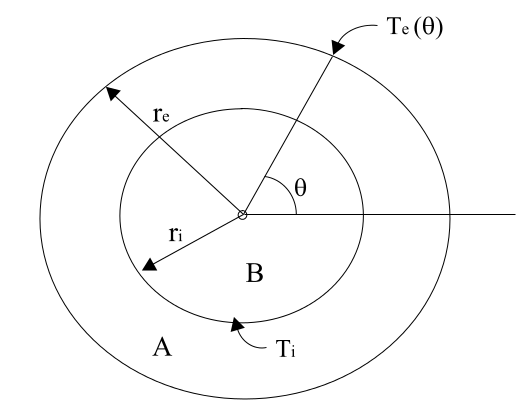
\includegraphics[width=0.6\columnwidth]{imagenes/horno.png}
\caption{Secci\'on circular del horno}
\end{center}
\end{figure}



El objetivo del trabajo práctico es implementar un programa que calcule la isoterma solicitada, conociendo las dimensiones del horno y las mediciones de temperatura en la pared exterior.

{\bf El Modelo}

Sea $r_e \in \mathbb{R}$ el radio exterior de la pared y sea $r_i \in \mathbb{R}$ el radio interior de la pared. Llamemos $T(r,\theta)$ a la temperatura en el punto dado por las coordenadas polares $(r,\theta)$, siendo $r$ el radio y $\theta$ el \'angulo polar de dicho punto. En el estado estacionario, esta temperatura satisface la ecuaci\'on del calor:

\begin{equation}\label{calor}
\frac{\partial^2T(r,\theta)}{\partial r^2}+\frac{1}{r}\frac{\partial T(r,\theta)}{\partial r}+\frac{1}{r^2}\frac{\partial^2T(r,\theta)}{\partial \theta^2} = 0 
\end{equation}


Si llamamos $T_i \in \mathbb{R}$ a la temperatura en el interior del horno (sector B) y $T_e : [0,2\pi] \rightarrow \mathbb{R}$ a la funci\'on de temperatura en el borde exterior del horno (de modo tal que el punto $(r_e,\theta)$ tiene temperatura $T_e(\theta)$), entonces tenemos que

\begin{equation}
T(r,\theta) = T_i \;\;\;\;\;para\;todo\;punto\;(r,\theta)\;con\;r\leq r_i
\end{equation}
\begin{equation}
T(r_e,\theta) = T_e(\theta) \;\;\;\;\;\;para\;todo\;punto\;(r_e,\theta)
\end{equation}


El problema en derivadas parciales dado por la primera ecuaci\'on con las condiciones de contorno presentadas recientemente, permite encontrar la funci\'on $T$ de temperatura en el interior del horno (sector A), en funci\'on de los datos mencionados en esta secci\'on.

Para resolver este problema computacionalmente, discretizamos el dominio del problema (el sector A) en coordenadas polares. Consideramos una partici\'on $0 = \theta_0 < \theta_1 < ... < \theta_n = 2\pi$ en $n$ \'angulos discretos con $\theta_k-\theta_{k-1} = \Delta\theta$ para $k = 1,...,n$, y una partici\'on $r_i = r_0 < r_1 < ... < r_m = r_e$ en $m+1$ radios discretos con $r_j - r_{j-1} = \Delta r$ para $j = 1,...,m$.

\medskip

El problema ahora consiste en determinar el valor de la funci\'on $T$ en los puntos de la discretizaci\'on $(r_j,\theta_k)$ que se encuentren dentro del sector A. Llamemos $t_{jk} = T(r_j,\theta_k)$ al valor (desconocido) de la funci\'on $T$ en el punto $(r_j,\theta_k)$.

\medskip

Para encontrar estos valores, transformamos la ecuaci\'on (\ref{calor}) en un conjunto de ecuaciones lineales sobre las inc\'ognitas $t_{jk}$, evaluando (\ref{calor}) en todos los puntos de la discretizaci\'on que se encuentren dentro del sector A. Al hacer esta evaluaci\'on, aproximamos las derivadas parciales de $T$ en (\ref{calor}) por medio de las siguientes f\'ormulas de diferencias finitas:


\begin{equation}
\frac{\partial^2T(r,\theta)}{\partial r^2}(r_j,\theta_k) \cong \frac{t_{j-1,k}-2t_{jk}+t_{j+1,k}}{(\Delta r)^2}
\end{equation}

\begin{equation}
\frac{\partial T(r,\theta)}{\partial r}(r_j,\theta_k) \cong \frac{t_{j,k}-t_{j-1,k}}{\Delta r}
\end{equation}

\begin{equation}
\frac{\partial^2T(r,\theta)}{\partial \theta^2}(r_j,\theta_k) \cong \frac{t_{j,k-1}-2t_{jk}+t_{j,k+1}}{(\Delta \theta)^2}
\end{equation}



Es importante notar que los valores de las inc\'ognitas son conocidos para los puntos que se encuentran sobre el borde exterior de la pared, y para los puntos que se encuentren dentro del sector B. Al realizar este procedimiento, obtenemos un sistema de ecuaciones lineales que modela el problema discretizado. La resoluci\'on de este sistema permite obtener una aproximaci\'on de los valores de la funci\'on $T$ en los puntos de la discretizaci\'on.

{\bf Enunciado}

Se debe implementar un programa en \verb+C+ o \verb-C++- que tome como entrada los par\'ametros del problema ($r_i$, $r_e$, $m+1$,
$n$, valor de la isoterma buscada, $T_i$, $T_e(\theta)$) que calcule la temperatura dentro de la pared del horno utilizando el
modelo propuesto en la secci\'on anterior y que encuentre la isoterma buscada en funci\'on del resultado obtenido del
sistema de ecuaciones. El m\'etodo para determinar la posici\'on de la isoterma queda a libre elecci\'on de cada grupo y
debe ser explicado en detalle en el informe.

El programa debe formular el sistema obtenido a partir de las ecuaciones (1) - (6) y considerar dos m\'etodos posibles
para su resoluci\'on: mediante el algoritmo cl\'asico de Eliminaci\'on Gaussiana y la Factorizaci\'on LU. Finalmente, el
programa escribir\'a en un archivo la soluci\'on obtenida con el formato especificado en la siguiente secci\'on.

Como ya se ha visto en la materia, no es posible aplicar los m\'etodos propuestos para la resoluci\'on a cualquier
sistema de ecuaciones. Sin embargo, la matriz del sistema considerado en el presente trabajo cumple con ser diagonal dominante (no
estricto) y que, ordenando las variables y ecuaciones convenientemente, es posible armar un sistema de ecuaciones cuya matriz
posee la propiedad de ser \emph{banda}. Luego, se pide demostrar (o al menos dar un esquema de la demostraci\'on)
el siguiente resultado e incluirlo en el informe:

\begin{proposition}
Sea $A \in \mathbb{R}^{n \times n}$ la matriz obtenida para el sistema definido por (1)-(6). Demostrar que es posible
aplicar Eliminaci\'on Gaussiana sin pivoteo.\footnote{Sugerencia: Notar que la matriz es diagonal dominante (no
estrictamente) y analizar qué sucede al aplicar un paso de Eliminaci\'on Gaussiana con los elementos de una fila.} 
\end{proposition}

La soluci\'on del sistema de ecuaciones permitir\'a saber la temperatura en los puntos de la discretizaci\'on. Sin embargo,
nuestro inter\'es es calcular la isoterma 500, para poder determinar si la estructura se encuentra en peligro. Luego, se pide lo siguiente:
\begin{itemize}
\item Dada la soluci\'on del sistema de ecuaciones, proponer una forma de estimar en cada \'angulo de la discretizaci\'on la posici\'on de la 
isoterma 500.
\item En funci\'on de la aproximaci\'on de la isoterma, proponer una forma (o medida) a utilizar para evaluar la peligrosidad de la estructura
en funci\'on de la distancia a la pared externa del horno.
\end{itemize}


En funci\'on de la experimentaci\'on, se busca realizar dos estudios complementarios: por un lado, analizar c\'omo se comporta el sistema y, por otro, 
cu\'ales son los requerimientos computacionales de los m\'etodos. Se pide como m\'inimo realizar los siguientes experimentos:
\begin{enumerate}
\item Comportamiento del sistema.
\begin{itemize}
\item Considerar al menos dos instancias de prueba, generando distintas discretizaciones para cada una de ellas y
comparando la ubicaci\'on de la isoterma buscada respecto de la pared externa del horno. Se sugiere presentar gr\'aficos
de temperatura o curvas de nivel para los mismos, ya sea utilizando las herramientas provistas por la c\'atedra o
implementando sus propias herramientas de graficaci\'on. 
\item Estudiar la proximidad de la isoterma buscada respecto de la pared exterior del horno en funci\'on de distintas 
granularidades de discretizaci\'on y las condiciones de borde. 
\end{itemize}
\item Evaluaci\'on de los m\'etodos.
\begin{itemize}
\item Analizar el tiempo de c\'omputo requerido para obtener la soluci\'on del sistema en funci\'on de la granularidad de 
la discretizaci\'on. Se sugiere presentar los resultados mediante gr\'aficos de tiempo de c\'omputo en funci\'on de alguna 
de las variables del problema.
\item Considerar un escenario similar al propuesto en el experimento 1. pero donde las condiciones de borde (i.e., $T_i$ y $T_e(\theta)$)
cambian en distintos instantes de tiempo. En este caso, buscamos obtener la secuencia de estados de la temperatura en
la pared del horno, y la respectiva ubicaci\'on de la isoterma especificada. Para ello, se considera una secuencia de $ninst$
vectores con las condiciones de borde, y las temperaturas en cada estado es la soluci\'on del correspondiente sistema de
ecuaciones. Se pide formular al menos un experimento de este tipo, aplicar los m\'etodos de resoluci\'on propuestos de
forma conveniente y compararlos en t\'erminos de tiempo total de c\'omputo requerido para distintos valores de $ninst$.
\end{itemize}
\end{enumerate}

De manera opcional, aquellos grupos que quieran ir un poco m\'as all\'a pueden considerar trabajar y desarrollar alguno(s) 
de los siguientes puntos extra:
\begin{enumerate}
\item Notar que el sistema resultante tiene estructura \emph{banda}. Proponer una estructura para aprovechar este hecho en t\'erminos de la
\emph{complejidad espacial} y como se adaptar\'ian los algoritmos de Eliminaci\'on Gaussiana y Factorizaci\'on LU para reducir la
cantidad de operaciones a realizar.
\item Implementar dicha estructura y las adaptaciones necesarias para el algoritmo de Eliminaci\'on Gaussiana.
\item Implementar dicha estructura y las adaptaciones necesarias para el algoritmo de Factorizaci\'on LU. 
\end{enumerate}

Finalmente, se deber\'a presentar un informe que incluya una descripci\'on detallada de los m\'etodos implementados y
las decisiones tomadas, el m\'etodo propuesto para el c\'alculo de la isoterma buscada y los experimentos realizados,
junto con el correspondiente an\'alisis y siguiendo las pautas definidas en el archivo \verb+pautas.pdf+.

{\bf Programa y formato de archivos}

Se deber\'an entregar los archivos fuentes que contengan la resoluci\'on del trabajo pr\'actico. El ejecutable tomar\'a
tres par\'ametros por l\'inea de comando, que ser\'an el archivo de entrada, el archivo de salida, y el m\'etodo a
ejectutar (0 EG, 1 LU).

El archivo de entrada tendr\'a la siguiente estructura:
\begin{itemize}
\item La primera l\'inea contendr\'a los valores $r_i$, $r_e$, $m+1$, $n$, $iso$, $ninst$, donde $iso$ representa el
valor de la isoterma buscada y $ninst$ es la cantidad de instancias del problema a resolver para los par\'ametros dados.
\item A continuaci\'on, el archivo contendr\'a $ninst$ l\'ineas, cada una de ellas con $2n$ valores, los primeros $n$ indicando los
valores de la temperatura en la pared interna, i.e., $T_i(\theta_0),T_i(\theta_1),\dots,T_i(\theta_{n-1})$, seguidos de $n$ valores
de la temperatura en la pared externa, i.e., $T_e(\theta_0)$,$T_e(\theta_1)$,$\dots$,$T_e(\theta_{n-1})$.
\end{itemize}

El archivo de salida obligatorio tendr\'a el vector soluci\'on del sistema reportando una componente del mismo por
l\'inea. En caso de $ninst > 1$, los vectores ser\'an reportados uno debajo del otro.

Junto con el presente enunciado, se adjunta una serie de scripts hechos en \verb+python+ y un conjunto instancias de
test que deber\'an ser utilizados para la compilaci\'on y un testeo b\'asico de la implementaci\'on. Se recomienda leer
el archivo \verb+README.txt+ con el detalle sobre su utilizaci\'on.

{\bf \underline{Fechas de entrega}}
\begin{itemize}
\item \emph{Formato Electr\'onico:} Jueves 3 de Septiembre de 2015, hasta las 23:59 hs, enviando el trabajo (informe +
c\'odigo) a la direcci\'on \verb+metnum.lab@gmail.com+. El subject del email debe comenzar con el texto \verb+[TP1]+
seguido de la lista de apellidos de los integrantes del grupo.
\item \emph{Formato f\'isico:} Viernes 4 de Septiembre de 2015, de 17:30 a 18:00 hs.
\end{itemize}

\noindent \textbf{Importante:} El horario es estricto. Los correos recibidos despu\'es de la hora indicada ser\'an
considerados re-entrega. Los grupos deben ser de 3 o 4 personas, sin excepci\'on. Es indispensable que los trabajos
pasen satisfactoriamente los casos de test provistos por la c\'atedra.


\newpage
\section{Código C++} \label{sec:codigo}
\subsection{alto_horno.h}
\lstinputlisting[language=C++]{codigo/alto-horno.h}
\subsection{alto_horno.cpp}
\lstinputlisting[language=C++]{codigo/alto-horno.cpp}
\subsection{sistema_ecuaciones.h}
\lstinputlisting[language=C++]{codigo/sistema-ecuaciones.h}
\subsection{sistema_ecuaciones.cpp}
\lstinputlisting[language=C++]{codigo/sistema-ecuaciones.cpp}


\end{document}
